%! TEX root = ../thesis.tex
\section{Model}
\label{kks:sec:model}

% Introduction to the section.
In this section, we formally introduce our probabilistic model.
For clarity, we take a clean-slate approach and develop the model from scratch.
We discuss in more detail how it relates to prior work in Section~\ref{kks:sec:relwork}.

% Features have latent score process that follows a GP
The basic building blocks of our model are \emph{features}\footnote{%
	In the simplest case, there is a one-to-one mapping between competitors (e.g., teams) and features, but decoupling them offers increased modeling power.}.
Let $M$ be the number of features; each feature $m \in [M]$ is characterized by a latent, continuous-time Gaussian process
\begin{align}
	\label{kks:eq:score}
	s_m(t) \sim \GP[0, k_m(t, t')].
\end{align}
We call $s_m(t)$ the \emph{score process} of $m$, or simply its \emph{score}.
The \emph{covariance function} of the process, $k_m(t, t') \doteq \Exp{s_m(t) s_m(t')}$, is used to encode time dynamics.
A brief introduction to Gaussian processes as well as a discussion of useful covariance functions is given in Section~\ref{kks:sec:covariances}.
The $M$ scores $s_1(t), \dots, s_M(t)$ are assumed to be (a priori) jointly independent, and we collect them into the \emph{score vector}
\begin{align*}
	\bm{s}(t) = \begin{bmatrix}s_1(t) & \cdots & s_M(t) \end{bmatrix}\Tr.
\end{align*}

% Competitors are sparse linear combination of M features
For a given match, each opponent $i$ is described by a sparse linear combination of the features, with coefficients $\bm{x}_i \in \mathbf{R}^M$.
That is, the score of an opponent $i$ at time $t^*$ is given by
\begin{align}
	\label{kks:eq:compscore}
	s_i = \bm{x}_i\Tr \bm{s}(t^*).
\end{align}
In the case of a one-to-one mapping between competitors and features, $\bm{x}_i$ is simply the one-hot encoding of opponent $i$.
More complex setups are possible: For example, in the case of team sports and if the player lineup is available for each match, it could also be used to encode the players taking part in the match~\citep{maystre2016player}.
Note that $\bm{x}_i$ can also depend contextually on the match.
For instance, it can be used to encode the fact that a team plays at home~\citep{agresti2012categorical}.

% Observations are parametrized by score difference.
Each observation consists of a tuple $(\bm{x}_i, \bm{x}_j, t^*, y)$, where $\bm{x}_i, \bm{x}_j$ are the opponents' feature vectors, $t^* \in \mathbf{R}$ is the time, and $y \in \mathcal{Y}$ is the match outcome.
We posit that this outcome is a random variable that depends on the opponents through their latent score difference:
\begin{align*}
	y \mid \bm{x}_i, \bm{x}_j, t^* \sim p( y \mid s_i - s_j ),
\end{align*}
where $p$ is a known probability density (or mass) function and $s_i, s_j$ are given by~\eqref{kks:eq:compscore}.
The idea of modeling outcome probabilities through score differences dates back to~\citet{thurstone1927law} and~\citet{zermelo1928berechnung}.
The likelihood $p$ is chosen such that positive values of $s_i - s_j$ lead to successful outcomes for opponent $i$ and vice-versa.

% Graphical representation.
A graphical representation of the model is provided in Figure~\ref{kks:fig:pgms}.
For perspective, we also include the representation of a static model, such as that of~\citet{thurstone1927law}.
Our model can be interpreted as ``conditionally parametric'': conditioned on a particular time, it falls back to a (static) pairwise-comparison model parametrized by real-valued scores.

\begin{figure}[t]
	\subcaptionbox{
		Static model
	}[2cm]{
		\begin{tikzpicture}

% Nodes.
\node[latent] (s)  {$s_m$};
\node[obs, below=of s] (y) {$y_n$};
\node[const, left=0.3cm of y, yshift=0.4cm] (x) {$\bm{x}_n$};

% Edges.
\edge {s} {y};
\edge[-] {x} {y};

% Plates.
\plate {scores} {(s)} {$M$}
\plate {observations} {(y)(x)} {$N$}
\end{tikzpicture}

	}
	\hfill
	\subcaptionbox{
		Our dynamic model \label{kks:fig:model}
	}{
		\begin{tikzpicture}

% Nodes.
\node[latent] (s1)  {$s_{m1}$};
\node[latent, right=1cm of s1] (s2)  {$s_{m2}$};
\node[latent, right=1.5cm of s2] (sn)  {$s_{mN}$};
\node[const, above=0.5cm of s1] (t1) {$t_1$};
\node[const, above=0.5cm of s2] (t2) {$t_2$};
\node[const, above=0.5cm of sn] (tn) {$t_N$};
\node[obs, below=of s1] (y1) {$y_1$};
\node[obs, below=of s2] (y2) {$y_2$};
\node[obs, below=of sn] (yn) {$y_N$};
\node[const, left=0.2cm of y1, yshift=0.4cm] (x1) {$\bm{x}_1$};
\node[const, left=0.3cm of y2, yshift=0.4cm] (x2) {$\bm{x}_2$};
\node[const, left=0.3cm of yn, yshift=0.4cm] (xn) {$\bm{x}_N$};

% Edges.
\edge[-] {t1} {s1};
\edge[-] {t2} {s2};
\edge[-] {tn} {sn};
\edge[-] {x1} {y1};
\edge[-] {x2} {y2};
\edge[-] {xn} {yn};
\edge {s1} {y1};
\edge {s2} {y2};
\edge {sn} {yn};

\path (t2) -- node[auto=false]{\ldots} (tn);
\path (y2) -- node[auto=false]{\ldots} (yn);
\draw[line width=2pt] (s1) -- (s2);
\draw[line width=2pt] (s2) -- node[fill=white] {\ldots} (sn);

% Plates.
\plate {scores} {(s1)(s2)(sn)} {$M$}
\end{tikzpicture}

	}
	\caption{
		Graphical representation of a static model (left) and of the dynamic model presented in this paper (right).
		The observed variables are shaded.
		For conciseness, we let $\bm{x}_n \doteq \bm{x}_{n,i} - \bm{x}_{n,j}$.
		Right: the latent score variables are mutually dependent across time, as indicated by the thick line.}
	\label{kks:fig:pgms}
\end{figure}

\paragraph{Observation Models}
Choosing an appropriate likelihood function $p(y \mid s_i - s_j)$ is an important modeling decision and depends on the information contained in the outcome $y$.
The most widely applicable likelihoods require only \emph{ordinal} observations, \textit{i.e.}, whether a match resulted in a win or a loss (or a tie, if applicable).
In some cases, we might additionally observe points (e.g., in association football, the number of goals scored by each team).
To make use of this extra information, we can model
\begin{enuminline}
	\item the number of points of opponent $i$ with a Poisson distribution whose rate is a function of $s_i - s_j$, or
	\item the points difference with a Gaussian distribution centered at $s_i - s_j$.
\end{enuminline}
A non-exhaustive list of likelihoods is given in Table~\ref{kks:tab:likelihoods}.

\begin{table}[t]
	\caption{
		Examples of observation likelihoods.
		The score difference is denoted by $d \doteq s_i - s_j$ and the Gaussian cumulative density function is denoted by $\Phi$.
	}
	\label{kks:tab:likelihoods}
	\centering
	\begin{tabular}{l lll}
		\toprule
		Name           & $\mathcal{Y}$        & $p(y \mid d)$                           & References                                      \\
		\midrule
		Probit         & $\{\pm 1 \}$         & $\Phi(yd)$                              & \citep{thurstone1927law, herbrich2006trueskill} \\
		Logit          & $\{\pm 1 \}$         & $[1 + \exp(-yd)]^{-1}$                  & \citep{zermelo1928berechnung, bradley1952rank}  \\
		Ordinal probit & $\{\pm 1, 0 \}$      & $\Phi(yd - \alpha), \ldots$             & \citep{glenn1960ties}                           \\
		Poisson-exp    & $\mathbf{N}_{\ge 0}$ & $\exp(yd - e^d) / y!$                   & \citep{maher1982modelling}                      \\
		Gaussian       & $\mathbf{R}$         & $\propto \exp[(y - d)^2 / (2\sigma^2)]$ & \citep{guo2012score}                            \\
		\bottomrule
	\end{tabular}
\end{table}


%%%%%%%%%%%%%%%%%%%%%%%%%%%%%%%%%
\subsection{Covariance Functions}
\label{kks:sec:covariances}

% Quick recap on Gaussian processes.
A Gaussian process $s(t) \sim \GP[0, k(t, t')]$ can be thought of as an infinite collection of random variables indexed by time, such that the joint distribution of any finite vector of $N$ samples $\bm{s} = [s(t_1) \cdots s(t_N)]$ is given by $\bm{s} \sim \mathcal{N}(\bm{0}, \bm{K})$, where $\bm{K} = [k(t_i, t_j)]$.
That is, $\bm{s}$ is jointly Gaussian with mean $\bm{0}$ and covariance matrix $\bm{K}$.
We refer the reader to~\citet{rasmussen2006gaussian} for an excellent introduction to Gaussian processes.

% Dynamics through covariance functions.
Hence, by specifying the covariance function appropriately, we can express prior expectations about the time dynamics of a feature's score, such as smooth or non-smooth variations at different timescales, regression to the mean, discontinuities, linear trends and more.
Here, we describe a few functions that we find useful in the context of modeling temporal variations.
Figure~\ref{kks:fig:covariances} illustrates these functions through random realizations of the corresponding Gaussian processes.

\begin{figure*}[t]
	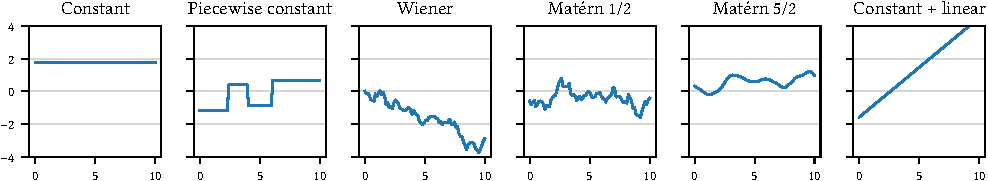
\includegraphics{kks-covariances}
	\caption{Random realizations of a zero-mean Gaussian process with six different covariance functions.}
	\label{kks:fig:covariances}
\end{figure*}

\begin{description}
	\item[Constant] This covariance captures processes that remain constant over time.
	      It is useful in composite covariances to model a constant offset (i.e., a mean score value).

	\item[Piecewise Constant]
	      Given a partition of $\mathbf{R}$ into disjoint intervals, this covariance is constant inside a partition and zero between partitions.
	      It can, for instance, capture discontinuities across seasons in professional sports leagues.

	\item[Wiener] This covariance reflects Brownian motion dynamics (c.f. Section~\ref{kks:sec:relwork}).
	      It is non-stationary: the corresponding process drifts away from $0$ as $t$ grows.

	\item[Matérn] This family of stationary covariance functions can represent smooth and non-smooth variations at various timescales.
	      It is parametrized by a variance, a characteristic timescale and a smoothness parameter $\nu$.
	      When $\nu = 1/2$, it corresponds to a mean-reverting version of Brownian motion.

	\item[Linear] This covariance captures linear dynamics.
\end{description}

% Composite covariance functions.
Finally, note that composite functions can be created by adding or multiplying covariance functions together.
For example, let $k_a$ and $k_b$ be constant and Matérn covariance functions, respectively.
Then, the composite covariance $k(t, t') \doteq k_a(t, t') + k_b(t, t')$ captures dynamics that fluctuate around a (non-zero) mean value.
\citet[Sec. 2.3]{duvenaud2014automatic} provides a good introduction to building expressive covariance functions by composing simple ones.
